\clearpage
\chapter{Study Guide 5}

\section{Linear Independence}
\horizontalline{0}{0}

\begin{center}
    \large{\textbf{Study Guide Instructions}}
\end{center}

\horizontalline{-1}{0}

\begin{itemize}
    \item Submit your work in Gradescope as a PDF - you will identify where your “questions are.”
    \item Identify the question number as you submit.  Since we grade "blind" if the questions are NOT identified, the work WILL NOT BE GRADED and a 0 will be recorded. Always leave enough time to 
    identify the questions when submitting.
    \item One section per page (if a page or less) - We prefer to grade the main solution in a single page, extra work can be included on the following page.
    \item Long instructions may be removed to fit on a single page.
    \item \textbf{Do not start a new question in the middle of a page.}
    \item Solutions to book questions are provided for reference.
    \item You may NOT submit given solutions - this includes minor modifications - as your own.
    \item Solutions that do not show individual engagement with the solutions will be marked as no credit and can be considered a violation of honor code.
    \item If you use the given solutions you must reference or explain how you used them, in particular...
\end{itemize}

\horizontalline{-1}{0}

\begin{center}
    \large{\textbf{Method Selection}}
\end{center}

\horizontalline{-1}{0}

\textbf{For full credit,  EACH book exercise in the Study Guides must use one or more of the following methods and FOR EACH QUESTION.  Identify the number the method by number to ensure full credit.}

\begin{itemize}
    \item \textbf{Method 1} - Provide original examples which demonstrate the ideas of the exercise in addition to your solution.
    \item \textbf{Method 2} - Include and discuss the specific topics needed from the chapter and how they relate to the question.
    \item \textbf{Method 3} - Include original Python code, of reasonable length (as screenshot or text)  to show how the topic or concept was explored.
    \item \textbf{Method 4} - Expand the given solution in a significant way, with additional steps and comments. All steps are justified. This is a good method for a proof for which you are only given a basic outline.
    \item \textbf{Method 5} - Attempt the exercise without looking at the solution and then the solution is used to check work. Words are used to describe the results.
    \item \textbf{Method 6} - Provide an analysis of the strategies used to understand the exercise, describing in detail what was challenging, who helped you or what resources were used. The process of understanding is
    described.
\end{itemize}

% Problem 1
\begin{problem}{Problem 1}
    \begin{statement}{Problem Statement}
        Pick a section of Chapter 5 to annotate.
    \end{statement}

    For annotations this week, I have chosen to annotate section 5.1 of VMLS. The annotations for this problem can be seen on the following page.

    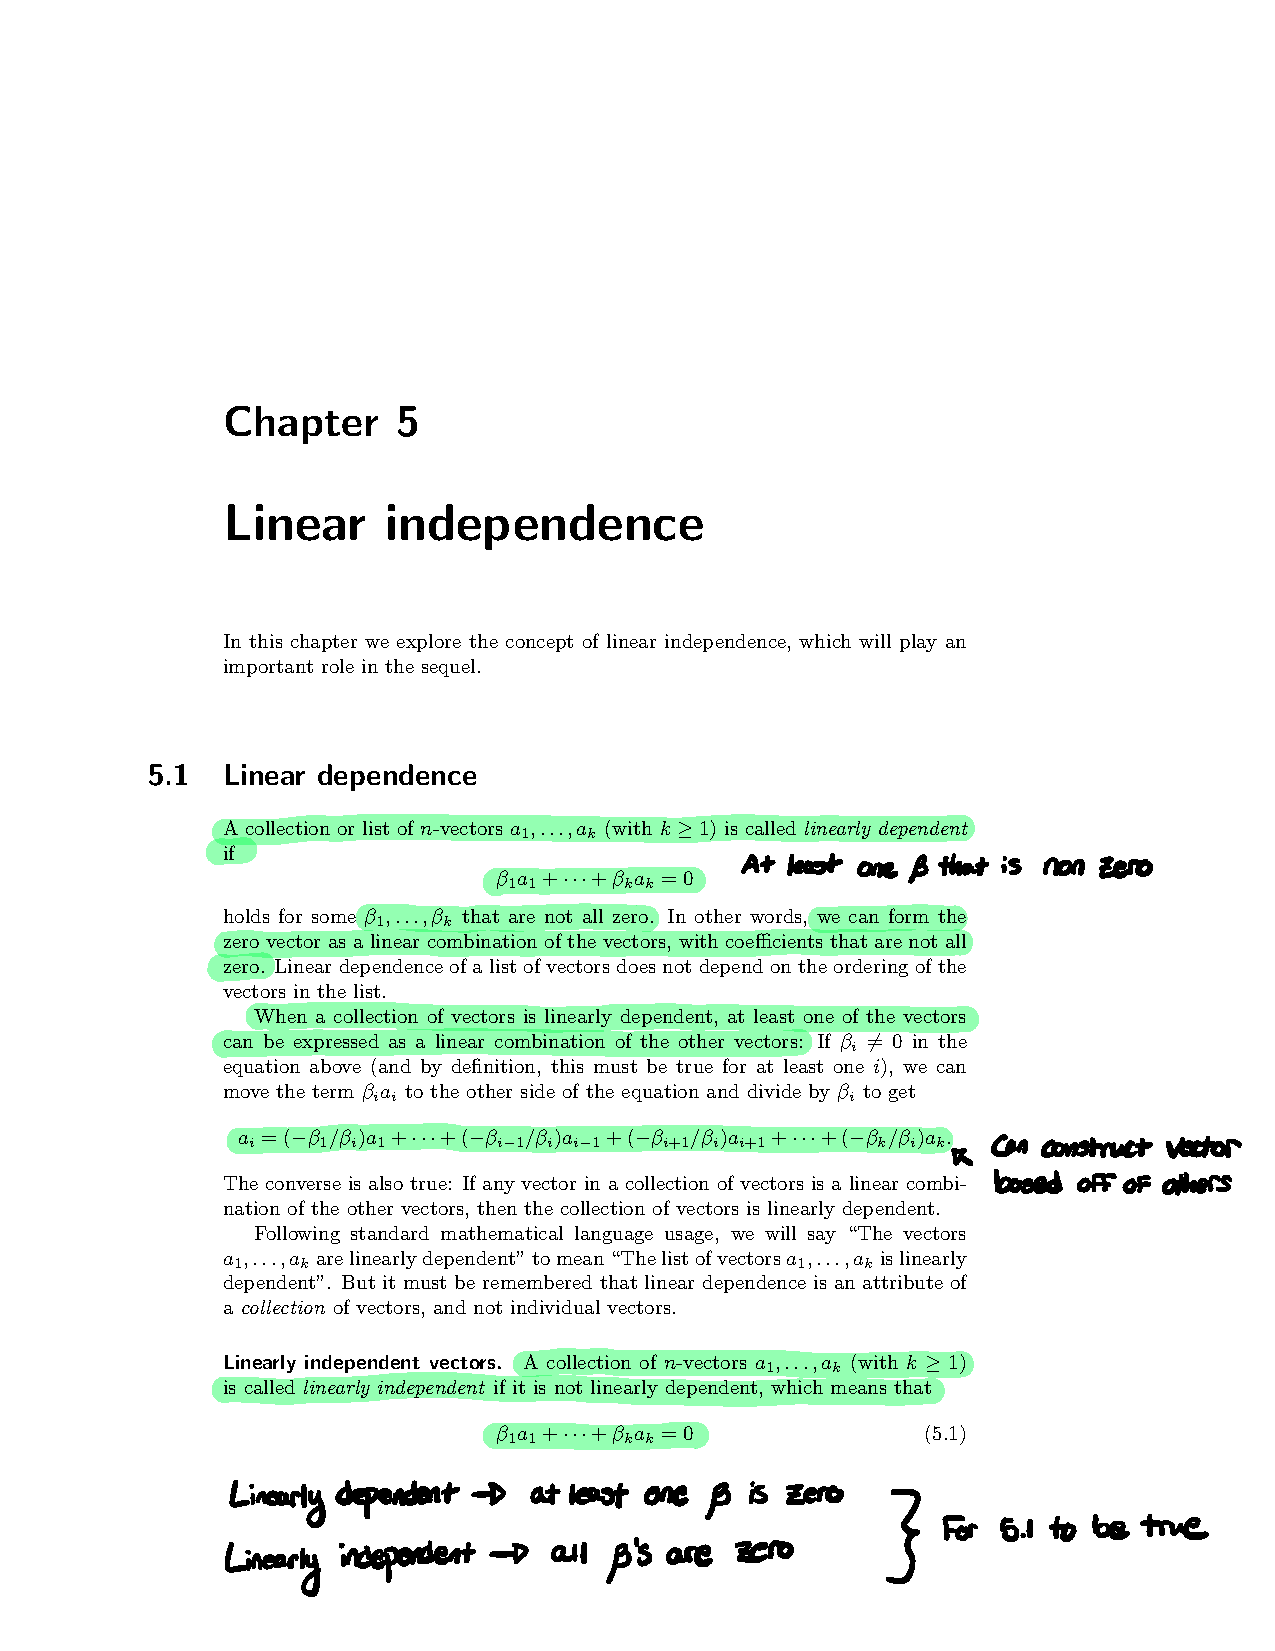
\includepdf[pages={-}, pagecommand={\thispagestyle{fancy}}, width=\paperwidth, offset=0 0]{./PDF/Annotations.pdf}
\end{problem}

% Problem 1 Summary
\begin{summary}{Problem 1 Summary}
    \begin{statement}{Procedure}
        \begin{itemize}
            \item Annotate a chapter from the textbook by adding notes and insights
        \end{itemize}
    \end{statement}
    \begin{statement}{Key Concepts}
        \begin{itemize}
            \item This chapter encapsulates what it means for a collection of vectors to be linearly independent or dependent
            \item For a collection of vectors to be linearly independent it must follow that
            \begin{equation*}
                \beta_{1}a_{1} + \dots + \beta_{k}a_{k} = 0
            \end{equation*}
            where the only way the above is true is if \textbf{every} $\beta$ is 0
            \item For a collection of vectors to be linearly dependent it must follow that 
            \begin{equation*}
                \beta_{1}a_{1} + \dots + \beta_{k}a_{k} = 0
            \end{equation*}
            where the above is true is if there is at least \textbf{one} $\beta$ that is non zero
        \end{itemize}
    \end{statement}
    \begin{statement}{Variations}
        \begin{itemize}
            \item We could be asked to annotate a different chapter or section of the textbook
        \end{itemize}
    \end{statement}
\end{summary}

% Problem 2
\begin{problem}{Problem 2}
    \begin{statement}{Problem Statement}
        Solve and explain the solution to 5.1 here in your own words. (Since you are given a solution, you will be graded on your ability to explain). \vspace*{1em}

        \textbf{Original Question:} \vspace*{1em}

        \textit{Linear independence of stacked vectors}. Consider the stacked vectors

        \begin{equation*}
            c_{1} = 
            \begin{bmatrix}
                a_{1} \\
                b_{1} \\
            \end{bmatrix}
            \hspace*{2pt} , \hspace*{2pt} \dots \hspace*{2pt} , \hspace*{2pt}
            c_{k} =
            \begin{bmatrix}
                a_{k} \\
                b_{k} \\
            \end{bmatrix}
            \hspace*{2pt} ,
        \end{equation*}
        where $a_{1}, \dots , a_{k}$ are $n$-vectors and $b_{1}, \dots , b_{k}$ are $m$-vectors.

        \begin{enumerate}[label = (\alph*)]
            \item Suppose $a_{1}, \dots , a_{k}$ are linearly independent. (We make no assumptions about the vectors $b_{1}, \dots , b_{k}$) Can we conclude that the stacked vectors $c_{1}, \dots , c_{k}$ 
            are linearly independent?
            \item Now suppose that $a_{1}, \dots , a_{k}$ are linearly dependent. (Again, with no assumptions about $b_{1}, \dots, b_{k}$.) Can we conclude that the stacked vectors $c_{1}, \dots , c_{k}$
            are linearly dependent?
        \end{enumerate}
    \end{statement}

    \begin{Highlight}[Solution - Part (a)]
        For this problem I will be using \textbf{Method 4}. \vspace*{1em}

        \textbf{VMLS Solution:}

        \begin{enumerate}[label = (\alph*)]
            \item Yes, the stacked vectors are always independent. Suppose that $\beta_{1} c_{1} + \dots + \beta_{k} c_{k} = 0$. Then we have $\beta_{1}a_{1} + \dots + \beta_{k} a_{k} = 0$ and $\beta_{1} 
            b_{1} + \dots + \beta_{k} b_{k} = 0$. Since $a_{1} , \dots , a_{k}$ are linearly independent, we must have $\beta_{1} = \dots = \beta_{k} = 0$. So $c_{1}, \dots , c_{k}$ are linearly 
            independent.
        \end{enumerate}

        \textbf{Explanation:} \vspace*{1em}

        We are told in the problem statement that the vector $a$ is linearly independent. Mathematically this means

        \setcounter{equation}{0}
        \begin{equation}
            \sum_{i = 1}^{k} \beta_{i}a_{i} = 0
        \end{equation}
        where the above is only valid if all values of $\beta$ are zero. This is the definition of linear independence. Now for the vector $b$ we have

        \begin{equation}
            \sum_{i = 1}^{k} \beta_{i}b_{i} = 0
        \end{equation}
        but the question is if all the values of $\beta$ in equation (2) are non-zero or zero. Applying a similar method to vector $c$ as we did to both vectors $a$ and $b$ we have

        \begin{equation}
            \sum_{i = 1}^{k} \beta_{i}c_{i} = 0
        \end{equation}
        where if we expand equation (3) we then have 

        \begin{equation}
            \sum_{i = 1}^{k} \beta_{i}c_{i} = \sum_{i = 1}^{k} \beta_{i}
            \begin{bmatrix}
                a_{i} \\
                b_{i} \\
            \end{bmatrix}
            = 0.
        \end{equation}
        Because the same $\beta$ is being multiplied to vector $b$ as it is to vector $a$, and we know that all the $\beta$'s must be zero for $a$ to be linearly independent, this implies that the 
        vector $c$ must also be \textit{\textbf{linearly independent}} as well.
    \end{Highlight}

    \begin{Highlight}[Solution - Part (b)]
        For this problem I will be using \textbf{Method 4}. \vspace*{1em}

        \textbf{VMLS Solution:}

        \begin{enumerate}[label = (\alph*), start = 2]
            \item No, we can’t conclude that they are dependent. We can find examples with $a_{i}$ linearly dependent, and $c_{i}$ linearly independent, and also examples with $a_{i}$ linearly 
            dependent, and $c_{i}$ linearly dependent. For the first example, take $a_{1} = a_{2} = 1$ (they are 1-vectors), and $b_{1} = 1 , b_{2} = 0$. For the second example, take the same $a_{i}$ 
            and $b_{1} = b_{2} = 1$.
        \end{enumerate}

        \textbf{Explanation:} \vspace*{1em}

        We are told in the problem statement that the vector $a$ is linearly dependent. Mathematically this means

        \begin{equation}
            \sum_{i = 1}^{k} \beta_{i}a_{i} = 0
        \end{equation}
        where for equation (5) to be true, there must be at least one value of $\beta$ that is non-zero for $a$ to be classified as linearly dependent. Because of this fact, we can't implicitly say
        whether or not vector $c$ is linearly independent or linearly dependent. There may still be a combination of values for $b$ to be considered linearly independent or dependent, and thus we can't
        conclude anything about vector $c$.

        Essentially, $b$ could be constructed in manner so that it is either linearly independent or linearly dependent and thus we can't make any direct assumptions about vector $c$. We could also have
        a length of $b$ that would violate the linear independence inequality as well.
    \end{Highlight}
\end{problem}

% Problem 2 Summary
\begin{summary}{Problem 2 Summary}
    \begin{statement}{Procedure}
        \begin{enumerate}[label = (\alph*)]
            \item Part (a)
            \begin{itemize}
                \item Show that if one collection of vectors is linearly independent we can conclude what the values of $\beta$ must be for both concatenated vectors
                \item Show that with this value of $\beta$ that both concatenated vectors are linearly independent and the entire vector is indeed linearly independent
            \end{itemize}
            \item Part (b)
            \begin{itemize}
                \item Show that if one collection of vectors is linearly dependent, this means that we can't deduce what the full vector is in terms of linearly independent and dependent because the 
                other vector is unknown
            \end{itemize}
        \end{enumerate}
    \end{statement}
    \begin{statement}{Key Concepts}
        \begin{itemize}
            \item If one vector is shown to be linearly independent in a stacked vector this then means that each vector is linearly independent and the entire vector is linearly independent
            \item If one vector is shown to be linearly dependent, we can't conclude what the stacked vector is linearly independent or dependent
        \end{itemize}
    \end{statement}
    \begin{statement}{Variations}
        \begin{itemize}
            \item We could be given a different set of stacked vectors where we are asked what the relationship between them is
            \begin{itemize}
                \item We then would need to reason what the coefficients of these vectors are to make a determination about the stacked vector
            \end{itemize}
        \end{itemize}
    \end{statement}
\end{summary}

% Problem 3
\begin{problem}{Problem 3}
    \begin{statement}{Problem Statement}
        Solve and Explain the solution to 5.2 here in your own words. (Since you are given a solution, you will be graded on your ability to explain). \vspace*{1em}

        \textbf{Original Question:} \vspace*{1em}

        \textit{A surprising discovery}. An intern at a quantitative hedge fund examines the daily returns of around 400 stocks over one year (which has 250 trading days). She tells her supervisor that 
        she has discovered that the returns of one of the stocks, Google (GOOG), can be expressed as a linear combination of the others, which include many stocks that are unrelated to Google (say, in a 
        different type of business or sector).

        Is the supervisor right? Did the intern make a mistake? Give a very brief explanation.
    \end{statement}

    \begin{Highlight}[Solution]
        For this problem I will be using \textbf{Method 4}. \vspace*{1em}

        \textbf{VMLS Solution:} \vspace*{1em}

        The supervisor is wrong, and the intern is most likely correct. She is examining 400 250-vectors, each representing the daily returns of a particular stock over one year. By the independence-dimension 
        inequality, any set of $n + 1$ or more $n$ vectors is linearly dependent, so we know that this set of vectors is linearly dependent. That is, there exist some vectors that can be expressed as a linear 
        combination of the others. It is quite likely that the returns of any particular stock, such as GOOG, can be expressed as a linear combination of the returns other stocks.

        Even if Google’s return can be expressed as a linear combination of the others, by the independence-dimension inequality, this fact is not as useful as it might seems. For example, Google’s future returns 
        would not be given by the same linear combination of other asset returns. So although the intern is right, and the supervisor is wrong, the observation cannot be monetized. \vspace*{1em}

        \textbf{Explanation:} \vspace*{1em}

        From VMLS, the independence-dimension equality is:

        \horizontalline{0}{0}

        \textbf{Independence-dimension inequality}. If the $n$-vectors $a_{1}, \dots , a_{k}$ are linearly independent, then $k \leq n$. In words:
        
        \begin{center}
            \textit{A linearly independent collection of n-vectors can have at most n elements.}
        \end{center}

        Put another way:
        
        \begin{center}
            \textit{Any collection of n + 1 or more n-vectors is linearly dependent.}
        \end{center}

        \horizontalline{-1}{0}

        From the problem statement, the intern is dealing with 400 (this is the value of $n$) 250-vectors (this is the value of $k$) that represent the returns of stocks for 400 different stocks. From the independence-inequality
        we know that this collection of vectors is \textit{\textbf{linearly dependent}} because $k = 250 \leq n = 400$.

        Translated to English, this means that the stock returns of one stock, for example GOOG in the problem statement, can be expressed as linear combinations of others. So, by this logic the intern is correct and the
        supervisor is wrong.
    \end{Highlight}
\end{problem}

% Problem 3 Summary
\begin{summary}{Problem 3 Summary}
    \begin{statement}{Procedure}
        \begin{itemize}
            \item Use the independence-dimension inequality to reason if the intern is correct
        \end{itemize}
    \end{statement}
    \begin{statement}{Key Concepts}
        \begin{itemize}
            \item Using the independence-dimension inequality we can reason that this collection of vectors is linearly dependent
            \item The independence-dimension inequality states that
            \begin{center}
                \textit{A linearly independent collection of n-vectors can have at most n elements.}
            \end{center}
            \begin{center}
                \textit{Any collection of n + 1 or more n-vectors is linearly dependent.}
            \end{center}
        \end{itemize}
    \end{statement}
    \begin{statement}{Variations}
        \begin{itemize}
            \item We could be given a different set of vectors to determine if they are linearly independent or dependent
            \begin{itemize}
                \item We would then reason with the independence-dimension inequality to determine if these vectors are linearly independent or dependent
            \end{itemize}
        \end{itemize}
    \end{statement}
\end{summary}

% Problem 4
\begin{problem}{Problem 4}
    \begin{statement}{Problem Statement}
        Solve and Explain the solution to 5.3 here in your own words. (Since you are given a solution, you will be graded on your ability to explain). \vspace*{1em}

        \textbf{Original Question:} \vspace*{1em}

        Replicating a cash flow with single-period loans. We continue the example described on page 93. Let $\mathbf{c}$ be any $\mathbf{n}$-vector representing a cash flow over $\mathbf{n}$ periods. Find the coefficients $\alpha_1, \ldots, \alpha_n$ of $\mathbf{c}$ in its expansion in the basis $\mathbf{e}_1, \mathbf{l}_1, \ldots, \mathbf{l}_{n-1}$, i.e.,

        \begin{equation*}
            \mathbf{c} = \alpha_1 \mathbf{e}_1 + \alpha_2 \mathbf{l}_1 + \ldots + \alpha_n \mathbf{l}_{n-1}.
        \end{equation*}
        Verify that $\alpha_1$ is the net present value (NPV) of the cash flow $\mathbf{c}$, defined on page 22, with interest rate $r$. Hint. Use the same type of argument that was used to show that $\mathbf{e}_1, \mathbf{l}_1, \ldots, \mathbf{l}_{n-1}$ are linearly independent. Your method will find $\alpha_n$ first, then $\alpha_{n-1}$, and so on.
    \end{statement}

    \begin{Highlight}[Solution]
        For this problem I will be using \textbf{Method 4}. \vspace*{1em}

        \textbf{VMLS Solution:} \vspace*{1em}

        As noted on page 93,

        \begin{equation*}
            \alpha_{1}e_{1} + \alpha_{2}l_{1} + \dots + \alpha_{n}l_{n - 1} = 
            \begin{bmatrix}
                \alpha_{1} + \alpha_{2} \\
                \alpha_{3} - (1 + r)\alpha_{2} \\
                \vdots \\
                \alpha_{n} - (1 + r)\alpha_{n - 1} \\
                -(1 + r)\alpha_{n} \\
            \end{bmatrix}.
        \end{equation*}
        We equate this to $c = (c_{1}, c_{2}, \dots, c_{n-1}, c_{n})$, and determine $\alpha_{n}, \alpha_{n - 1}, \dots, \alpha_{1}$ from the equality:

        \begin{equation*}
            \alpha_{n} = -\frac{c_{n}}{1 + r},
        \end{equation*}
        and therefore

        \begin{equation*}
            \alpha_{n - 1} = -\frac{c_{n - 1} - \alpha_{n}}{1 + r} = -\frac{c_{n - 1}}{1 + r} - \frac{c_{n}}{(1 + r)^2},
        \end{equation*}
        and 

        \begin{equation*}
            \alpha_{n - 2} = -\frac{c_{n -2} - \alpha_{n - 1}}{1 + r} = -\frac{c_{n - 2}}{1 + r} - \frac{c_{n - 1}}{(1 + r)^{2}} - \frac{c_{n}}{(1 + r)^{2}},
        \end{equation*}
        et cetera. Continuing the pattern we find

        \begin{equation*}
            \alpha_{2} = -\frac{c_{2}}{1 + r} -\frac{c_{3}}{(1 + r)^{2}} - \dots - \frac{c_{n}}{(1 + r)^{n-1}}
        \end{equation*}
        and finally

        \begin{equation*}
            \alpha_{1} = c_{1} - \alpha_{2} = c_{1} + \frac{c_{2}}{1 + r} + \dots + \frac{c_{n}}{(1 + r)^{n - 1}}.
        \end{equation*}
        This is exactly the net present value (NPV) of the cash flow, with interest rate $r$.
    \end{Highlight}
\end{problem}

% Problem 4 Summary
\begin{summary}{Problem 4 Summary}
    \begin{statement}{Procedure}
        \begin{itemize}
            \item Follow the logic of the VMLS solution
        \end{itemize}
    \end{statement}
    \begin{statement}{Key Concepts}
        \begin{itemize}
            \item This proof is used to show that $\alpha_{1}$ is the NPV of the cash flow
        \end{itemize}
    \end{statement}
    \begin{statement}{Variations}
        \begin{itemize}
            \item We could be given a different expression to prove
            \begin{itemize}
                \item We would then need to use proper algebra and whatnot to reach the new conclusion
            \end{itemize}
        \end{itemize}
    \end{statement}
\end{summary}

% Problem 5 
\begin{problem}{Problem 5}
    \begin{statement}{Problem Statement}
        Solve and Explain the solution to 5.4 here in your own words. (Since you are given a solution, you will be graded on your ability to explain). \vspace*{1em}

        \textbf{Original Question:} \vspace*{1em}

        \textit{Norm of linear combination of orthonormal vectors}. Suppose $a_{1}, \dots , a_{k}$ are orthonormal $n$-vectors, and $x = \beta_{1}a_{1} + \dots + \beta_{k}a_{k}$, where $\beta_{1}, 
        \dots , \beta_{k}$ are scalars. Express $\| x \|$ in terms of $\beta = (\beta_{1}, \dots , \beta_{k})$.
    \end{statement}

    \begin{Highlight}[Solution]
        For this problem I will be using \textbf{Method 4}. \vspace*{1em}

        \textbf{VMLS Solution:}

        \begin{align*}
            \| x \|^{2} & = x^{T}x \\
            & = (\beta_{1}a_{1} + \dots + \beta_{k}a_{k})^{T}(\beta_{1}a_{1} + \dots + \beta_{k}a_{k}) \\
            & = \beta_{1}^{2} + \dots + \beta_{k}^{2} \\
            & = \| \beta \|^{2}.
        \end{align*}
        (Going from the third to the fourth expression we use $a_{i}^{T}a_{i} = 1$, $a_{i}^{T}a_{j} = 0$ for $j \neq i$.) So we have the simple formula $\|x\| = \|\beta\|$.
    \end{Highlight}
\end{problem}

% Problem 5 Summary
\begin{summary}{Problem 5 Summary}
    \begin{statement}{Procedure}
        \begin{itemize}
            \item Use the definition of inner product to reach the conclusion
        \end{itemize}
    \end{statement}
    \begin{statement}{Key Concepts}
        \begin{itemize}
            \item The inner product of orthonormal vectors will evaluate to just the norm of the coefficients
        \end{itemize}
    \end{statement}
    \begin{statement}{Variations}
        \begin{itemize}
            \item We could be given a different type of vectors to show what the relationship of them is
            \begin{itemize}
                \item We would then have to use the proper definitions and whatnot to show this final relationship
            \end{itemize}
        \end{itemize}
    \end{statement}
\end{summary}

% Problem 6
\begin{problem}{Problem 6}
    \begin{statement}{Problem Statement}
        Solve and Explain the solution to 5.5 here in your own words. (Since you are given a solution, you will be graded on your ability to explain). \vspace*{1em}

        \textbf{Original Question} \vspace*{1em}

        \textit{Orthogonalizing vectors}. Suppose that $a$ and $b$ are any $n$-vectors. Show that we can always find a scalar $\gamma$ so that $(a - \gamma b) \perp b$, and that $\gamma$ is unique if 
        $b \neq 0$. (Give a formula for the scalar $\gamma$.) In other words, we can always subtract a multiple of a vector from another one, so that the result is orthogonal to the original vector. 
        The orthogonalization step in the Gram–Schmidt algorithm is an application of this.
    \end{statement}

    \begin{Highlight}[Solution]
        For this problem I will be using \textbf{Method 4}. \vspace*{1em}

        Two vectors are orthogonal if their inner product is zero. So we want to find $\gamma$ such that $(a - \gamma b)^{T}b = a^{T}b - \gamma b^{T}b = 0$. If $b = 0$, then we can choose any $\gamma$, 
        and we have $(a - \gamma b) \perp b$, since all vectors are orthogonal to 0. If $b \neq 0$, then $b^{T}b = \| b \|^{2} \neq 0$, and we can take $\gamma = a^{T}b / b^{T}b$. \vspace*{1em}

        \textbf{Explanation:} \vspace*{1em}

        We know that two vectors (in this case lets call them $\alpha$ and $\beta$) are said to be orthogonal if their inner product is zero. Namely,

        \setcounter{equation}{0}
        \begin{equation}
            \alpha^{T}\beta = 0.
        \end{equation}
        So, from the problem statement this means that

        \begin{equation}
            (a - \gamma b)^{T}b = 0
        \end{equation}
        must be true. Expanding equation (2) we then have

        \begin{align}
            (a - \gamma b)^{T}b & = 0 & \text{(Premise)} \\
            (a^{T} - \gamma b^{T})b & = 0 & \text{(Distribution of transpose)} \\
            a^{T}b - \gamma b^{T}b & = 0  & \text{(Distribution of inner product)} \\
            a^{T}b & = \gamma b^{T}b & \text{(Simplification by addition)} \\
            \frac{a^{T}b}{b^{T}b} & = \gamma & \text{(Simplification by division)} \\
            \gamma & = \frac{a^{T}b}{b^{T}b} & \text{(Commutative property)}
        \end{align}
        where equation (8) is the result of several operations involving inner products. These operations are valid by the distributivity property of transposes and since inner products of vectors are 
        scalar values. It should be noted that the result in equation (8) is only valid if $b$ is not the zero vector. This of course means that our value for $\gamma$ is then

        \begin{equation}
            \gamma = \frac{a^{T}b}{b^{T}b}.
        \end{equation}
    \end{Highlight}
\end{problem}

% Problem 6 Summary
\begin{summary}{Problem 6 Summary}
    \begin{statement}{Procedure}
        \begin{itemize}
            \item Use the definition of orthogonal to show what the inner product must evaluate to
            \item Use the distributive property of transposes and inner products with algebra to solve for $\gamma$
        \end{itemize}
    \end{statement}
    \begin{statement}{Key Concepts}
        \begin{itemize}
            \item We can find a scalar value in this inner product relationship with the use of properties and algebra
        \end{itemize}
    \end{statement}
    \begin{statement}{Variations}
        \begin{itemize}
            \item We could be asked to find this value for a different condition of vectors
            \begin{itemize}
                \item We would then use the properties of whatever is handed to us to find this value
            \end{itemize}
        \end{itemize}
    \end{statement}
\end{summary}

% Problem 7
\begin{problem}{Problem 7}
    \begin{statement}{Problem Statement}
        Solve and Explain the solution to 5.6 here in your own words. (Since you are given a solution, you will be graded on your ability to explain). \vspace*{1em}

        \textbf{Original Question:} \vspace*{1em}

        \textit{Gram–Schmidt algorithm}. Consider the list of $n$ $n$-vectors 

        \begin{equation*}
            a_{1} = 
            \begin{bmatrix}
                1 \\
                0 \\
                0 \\
                \vdots \\
                0 \\
            \end{bmatrix}
            \hspace*{2pt} , \hspace*{2pt}
            a_{2} = 
            \begin{bmatrix}
                1 \\
                1 \\
                0 \\
                \vdots \\
                0 \\
            \end{bmatrix}
            \hspace*{2pt} , \hspace*{2pt} \dots , \hspace*{2pt}
            a_{n} = 
            \begin{bmatrix}
                1 \\
                1 \\
                1 \\
                \vdots \\
                1 \\
            \end{bmatrix}.
        \end{equation*}
        (The vector $a_{i}$ has its first $i$ entries equal to one, and the remaining entries zero.) Describe what happens when you run the Gram–Schmidt algorithm on this list of vectors, i.e., say 
        what $q_{1}, \dots , q_{n}$ are. Is $a_{1}, \dots , a_{n}$ a basis?
    \end{statement}

    \begin{Highlight}[Solution]
        For this problem I will be using \textbf{Method 4}. \vspace*{1em}

        \textbf{VMLS Solution:} \vspace*{1em}

        $\tilde{q}_{1} = a_{1}$ has norm one, so we have $q_{1} = a_{1} = e_{1}$. $\tilde{q}_{2} = a_{2} - (q_{1}^{T}a_{2})q_{2} = e_{2}$ also has norm one, so $q_{2} = e_{2}$. This pattern continues,
        and we see that $q_{i} = e_{i}$.

        Yes, they are a basis. We know this since the Gram–Schmidt algorithm terminates after processing all $n$ vectors. We can also see this directly. Suppose that $\beta_{1}a_{1} + \dots + 
        \beta_{n}a_{n} = 0$. The last entry of this vector is $\beta_{n}$, so we know that $\beta_{n} = 0$. This implies that $\beta_{1}a_{1} + \dots + \beta_{n - 1}a_{n - 1} = 0$. The ($n - 1$) entry
        of this vector is $\beta_{n - 1}$, so we know that $\beta_{n - 1} = 0$. This continues, and we conclude that all $\beta_{i}$ are zero. So the vectors are linearly independent, and therefore a basis. \vspace*{1em}

        \textbf{Explanation:} \vspace*{1em}

        The first step of the Gram–Schmidt algorithm is orthogonalization. Namely,

        \setcounter{equation}{0}
        \begin{equation}
            \tilde{q}_{i} = a_{i} - \sum_{j = 1}^{i - 1} (q_{j}^{T}a_{i})q_{j}.
        \end{equation}
        From a quick inspection of $a_{1}$ we can see that $a_{1}$ is the unit vector $e_{1}$. If we then move on to $a_{2}$ we see

        \begin{align}
            \tilde{q}_{2} & = a_{2} - \sum_{j = 1}^{i - 1} (q_{j}^{T}a_{i})q_{j} \\
            & = a_{2} - \Bigg( (q_{1}^{T}a_{2})q_{1} \Bigg) \\
            & = 
            \begin{bmatrix}
                1 \\
                1 \\
                0 \\
                \vdots \\
                0 \\
            \end{bmatrix}
            - \Bigg(
            \begin{bmatrix}
                1 & 0 & 0 & \dots & 0 \\
            \end{bmatrix}
            \times
            \begin{bmatrix}
                1 \\
                1 \\
                0 \\
                \vdots \\
                0 \\
            \end{bmatrix}
            \Bigg)
            \begin{bmatrix}
                1 \\
                1 \\
                0 \\
                \vdots \\
                0 \\
            \end{bmatrix} 
            = 
            \begin{bmatrix}
                1 \\
                1 \\
                0 \\
                \vdots \\
                0 \\
            \end{bmatrix}
            - (1)
            \begin{bmatrix}
                1 \\
                0 \\
                0 \\
                \vdots \\
                0 \\
            \end{bmatrix}
            =
            \begin{bmatrix}
                0 \\
                1 \\
                0 \\
                \vdots \\
                0 \\
            \end{bmatrix}
            = e_{2}.
        \end{align}
        Just as $q_{1}$ was the unit vector $e_{1}$, we see that $q_{2}$ is also a unit vector $e_{2}$. One can infer that this pattern will repeat for all vectors $a_{i}$ and thus each vector $a_{i}$ 
        is a unit vector. Namely,

        \begin{equation}
            \tilde{q}_{i} = e_{i}.
        \end{equation}

        Now, since each $\tilde{q}_{i}$ is a unit vector, the only way that 

        \begin{equation}
            \sum_{i = i}^{n} \beta_{i}\tilde{q}_{i} = 0
        \end{equation}
        is a true statement is if all values of $\beta$ are zero. This implies that the vectors $\tilde{q}_{i}$ are \textit{\textbf{linearly independent}}. This further implies that $a_{i}$ form a basis.
    \end{Highlight}
\end{problem}

% Problem 7 Summary
\begin{summary}{Problem 7 Summary}
    \begin{statement}{Procedure}
        \begin{itemize}
            \item Use the Gram–Schmidt algorithm to find what these vectors will evaluate to in the given collection
        \end{itemize}
    \end{statement}
    \begin{statement}{Key Concepts}
        \begin{itemize}
            \item For this given set of vectors we can show that after the first step of Gram–Schmidt the vectors are unit vectors
        \end{itemize}
    \end{statement}
    \begin{statement}{Variations}
        \begin{itemize}
            \item We could be given a different set of vectors and be asked to use the Gram–Schmidt algorithm on them
            \begin{itemize}
                \item We would then use the Gram–Schmidt algorithm on them and conclude what they are after
            \end{itemize}
        \end{itemize}
    \end{statement}
\end{summary}